\section{Report di Qualità del Codice}
    \begin{figure}[H]
        \centering
        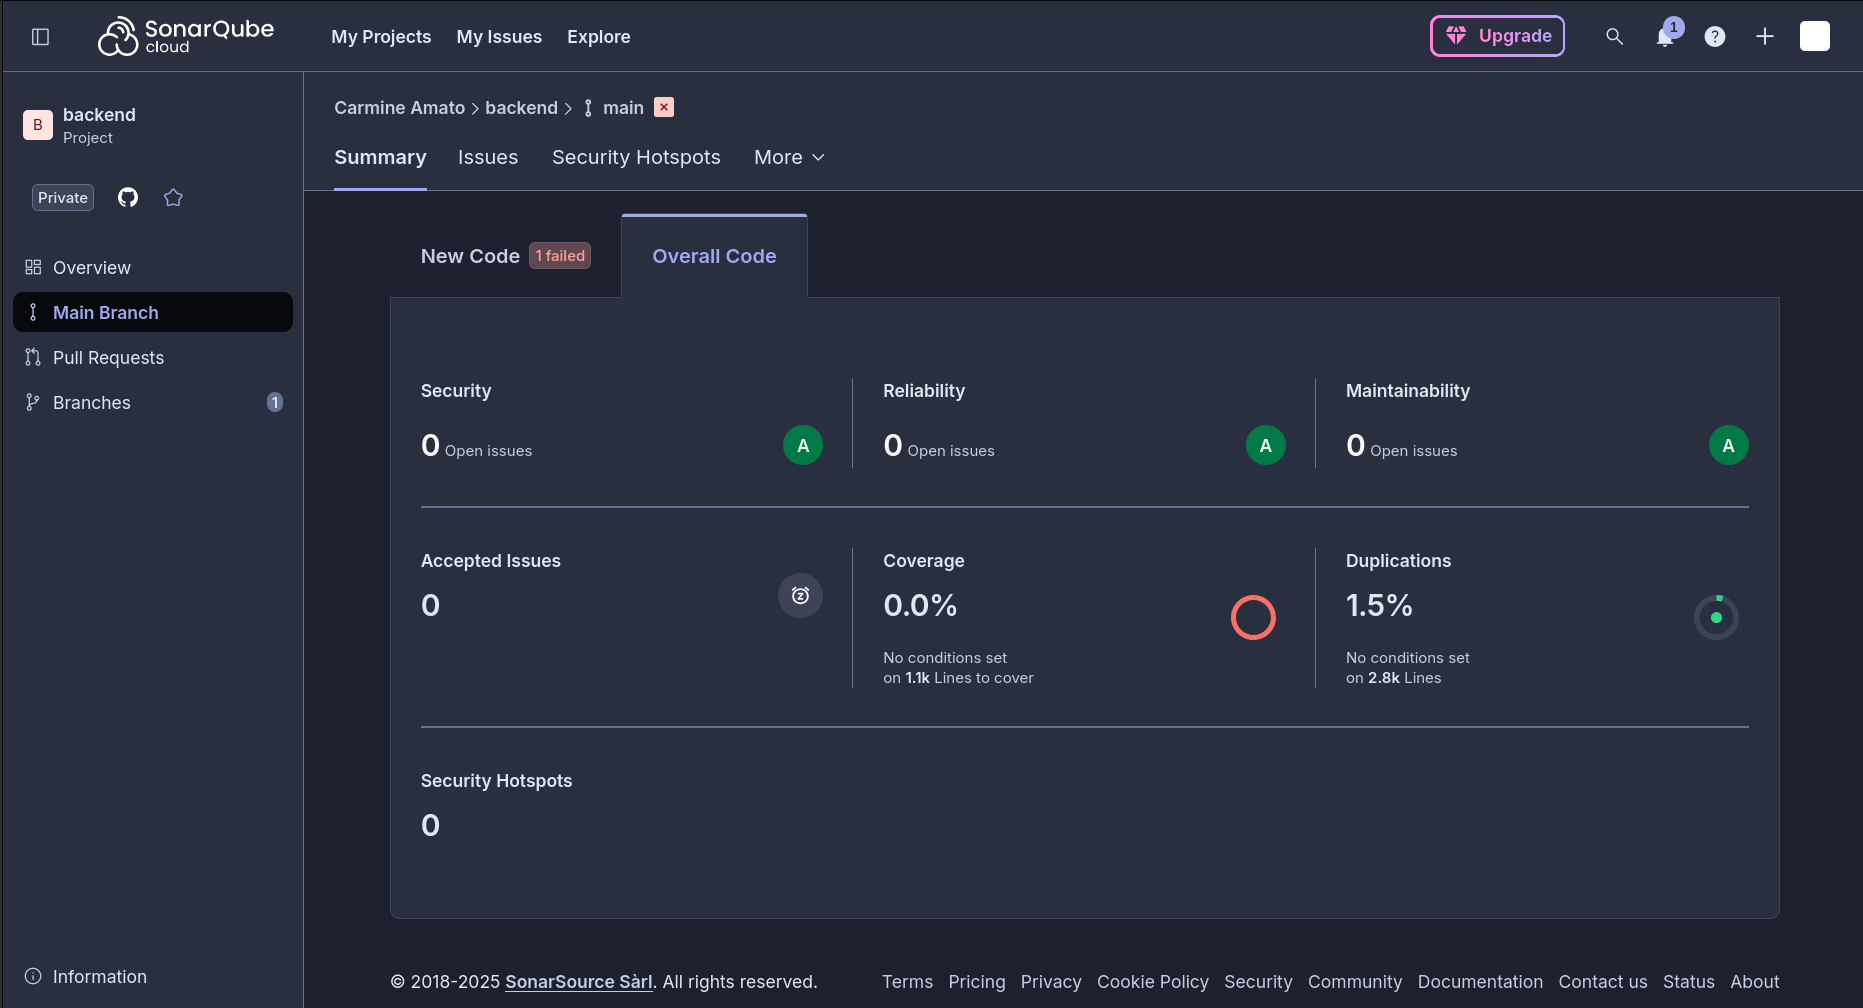
\includegraphics[width=0.8\linewidth]{src/report-qualità-codice/QualityReport.png}
        \caption{Report di Qualità da Sonar Qube Cloud}\label{QualityReport}
    \end{figure}

    Per avere costante contezza della qualità del codice scritto, ci siamo serviti di 
    SonarQube Cloud e SonarQube (attraverso estensione per IDE).

    \begin{figure}[H]
        \centering
        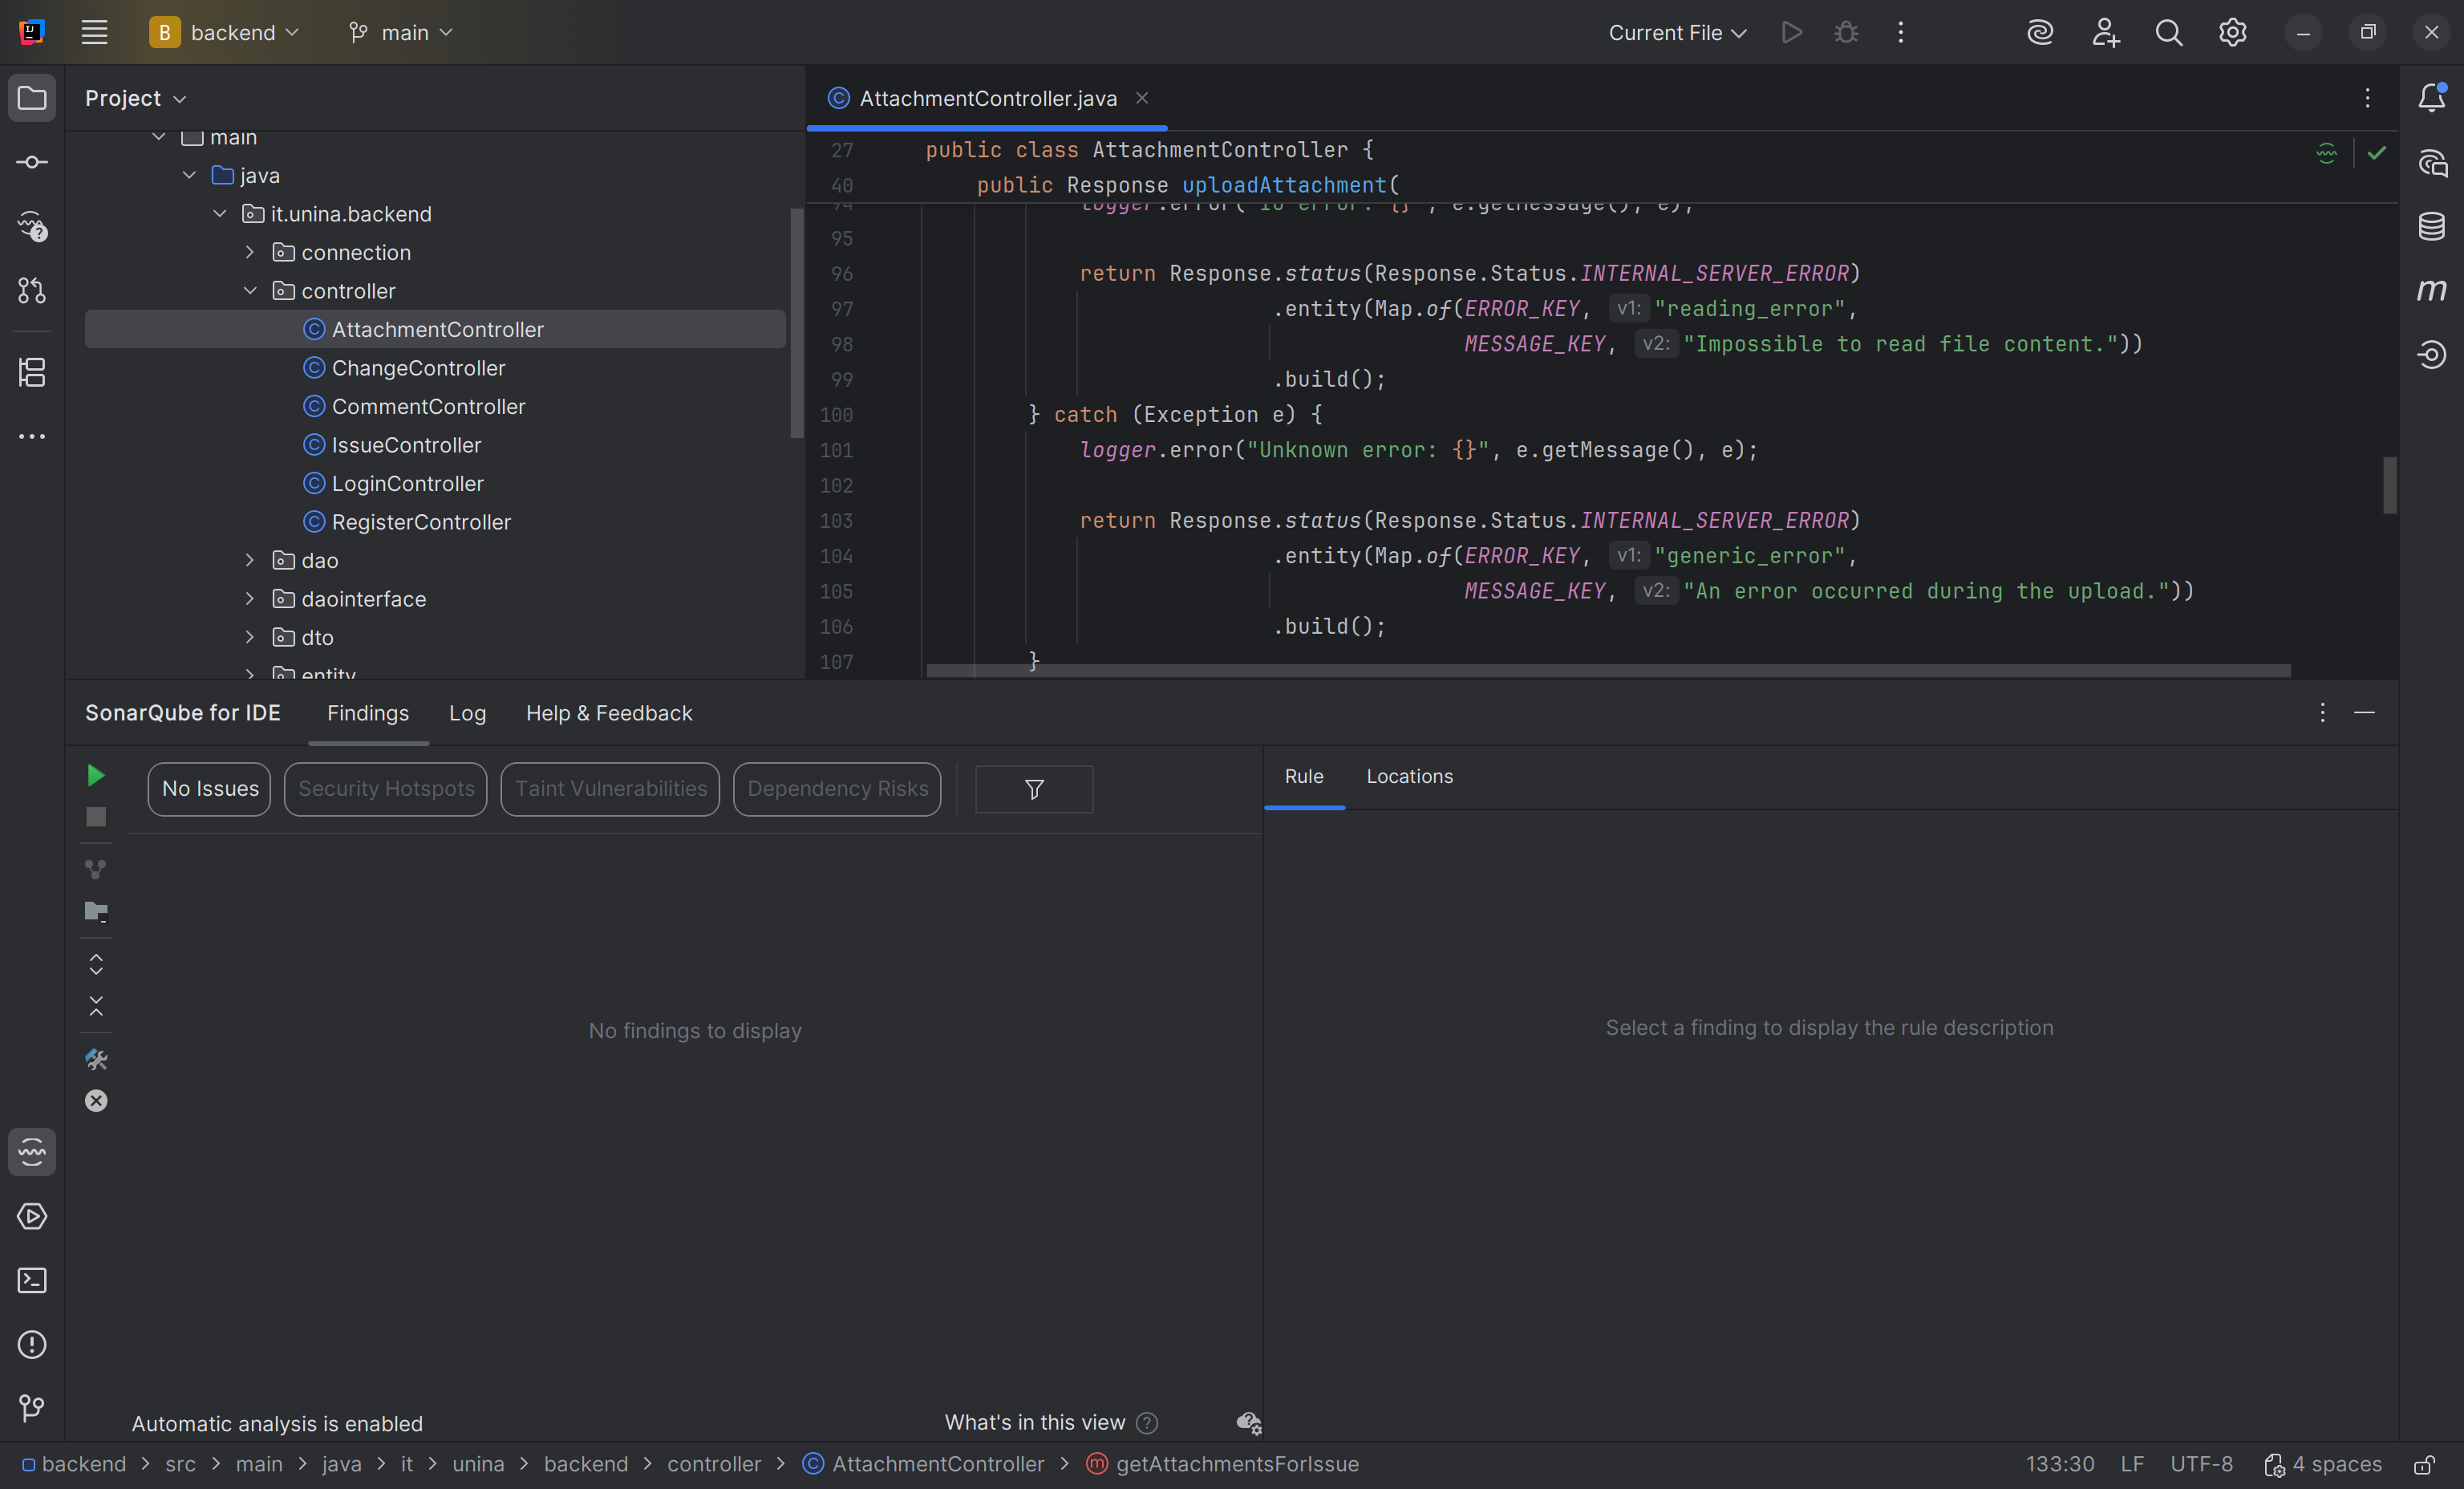
\includegraphics[width=0.8\linewidth]{src/report-qualità-codice/SonarQubeIDE.png}
        \caption{Esempio di Utilizzo di SonarQube for IDE su Intellij IDEA}\label{SonarQubeIDE}
    \end{figure}